
\documentclass[border=8pt, multi, tikz]{standalone} 
\usepackage{import}
\subimport{../../layers/}{init}
\usetikzlibrary{positioning}
\usetikzlibrary{3d} %for including external image 

\def\ConvColor{rgb:yellow,5;red,2.5;white,5}
\def\ConvReluColor{rgb:yellow,5;red,5;white,5}
\def\PoolColor{rgb:red,1;black,0.3}
\def\UnpoolColor{rgb:blue,2;green,1;black,0.3}
\def\FcColor{rgb:blue,5;red,2.5;white,5}
\def\FcReluColor{rgb:blue,5;red,5;white,4}
\def\FcFineColor{rgb:green,10;red,2.5;black,3}
\def\FcReluFineColor{rgb:green,10;red,6.5;black,3}
\def\SoftmaxColor{rgb:green,10;black,7}   
\def\SumColor{rgb:blue,5;green,15}

\newcommand{\copymidarrow}{\tikz \draw[-Stealth,line width=0.8mm,draw={rgb:blue,4;red,1;green,1;black,3}] (-0.3,0) -- ++(0.3,0);}

\begin{document}
\begin{tikzpicture}
\tikzstyle{connection}=[ultra thick,every node/.style={sloped,allow upside down},draw=\edgecolor,opacity=0.7]
\tikzstyle{copyconnection}=[ultra thick,every node/.style={sloped,allow upside down},draw={rgb:blue,4;red,1;green,1;black,3},opacity=0.7]

\pic[shift={(0,0,0)}] at (0,0,0) 
    {Box={
        name=input,
        caption=input,
        xlabel=3,
        ylabel=32,
        zlabel=32,
        fill=\ConvColor,
        height=32,
        width=3,
        depth=32
        }
    };

\node[canvas is zy plane at x=0] (temp) at (input-east) {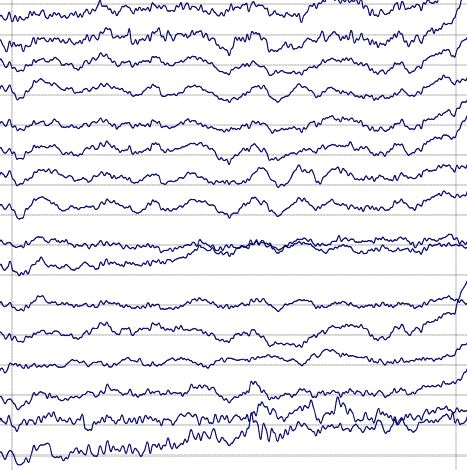
\includegraphics[width=6cm,height=6cm]{eeg.jpg}};

\pic[shift={(3,0,0)}] at (input-east) 
    {RightBandedBox={
        name=conv1,
        caption=conv1,
        xlabel=6,
        ylabel=28,
        zlabel=28,
        fill=\ConvColor,
        bandfill=\ConvReluColor,
        height=28,
        width=6,
        depth=28
        }
    };

\draw [connection]  (input-east)    -- node {\midarrow} (conv1-west);

\pic[shift={ (0,0,0) }] at (conv1-east) 
    {Box={
        name=pool1,
        caption=AvgPool,
        xlabel=6,
        ylabel=14,
        zlabel=14,    
        fill=\PoolColor,
        opacity=0.5,
        height=14,
        width=6,
        depth=14
        }
    };

\pic[shift={(2,0,0)}] at (pool1-east) 
    {RightBandedBox={
        name=conv2,
        caption=conv2,
        xlabel=8,
        ylabel=10,
        zlabel=10,
        fill=\ConvColor,
        bandfill=\ConvReluColor,
        height=10,
        width=8,
        depth=10
        }
    };

\draw [connection]  (pool1-east)    -- node {\midarrow} (conv2-west);

\pic[shift={ (0,0,0) }] at (conv2-east) 
    {Box={
        name=pool21,
        caption=AvgPool,
        xlabel=8,
        ylabel=5,
        zlabel=5,    
        fill=\PoolColor,
        opacity=0.5,
        height=5,
        width=8,
        depth=5
        }
    };

\pic[shift={(5,0,0)}] at (pool21-east) 
    {Box={
        name=input1,
        caption=frame1,
        xlabel=1,
        ylabel=1,
        zlabel=200,
        fill=\ConvColor,
        height=2.5,
        width=2.5,
        depth=100
        }
    };

\pic[shift={ (6,0,0) }] at (input1-east) 
    {Box={
        name=node11,
        caption=,
        xlabel=1,
        ylabel=1,
        zlabel=16,
        fill=\FcColor,
        height=2.5,
        width=2.5,
        depth=8
        }
    };

\pic[shift={ (3,0,0) }] at (node11-east) 
    {Box={
        name=node21,
        caption=,
        xlabel=1,
        ylabel=1,
        zlabel=16,
        fill=\FcColor,
        height=2.5,
        width=2.5,
        depth=8
        }
    };

\pic[shift={ (3,0,0) }] at (node21-east) 
    {Box={
        name=node31,
        caption=,
        xlabel=1,
        ylabel=1,
        zlabel=16,
        fill=\FcColor,
        height=2.5,
        width=2.5,
        depth=8
        }
    };

\draw [connection]  (pool21-east)    -- node {\midarrow} (input1-west);

\draw [connection]  (input1-east)    -- node {\midarrow} (node11-west);

\draw [connection]  (node11-east)    -- node {\midarrow} (node21-west);

\draw [connection]  (node21-east)    -- node {\midarrow} (node31-west);

\pic[shift={(0,-10,0)}] at (0,0,0) 
    {Box={
        name=input,
        caption=input,
        xlabel=3,
        ylabel=32,
        zlabel=32,
        fill=\ConvColor,
        height=32,
        width=3,
        depth=32
        }
    };

\node[canvas is zy plane at x=0] (temp) at (input-east) {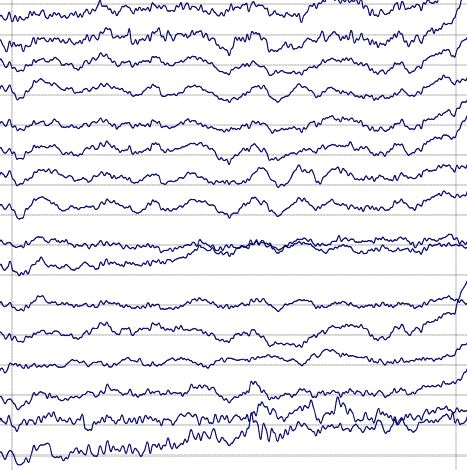
\includegraphics[width=6cm,height=6cm]{eeg.jpg}};

\pic[shift={(3,0,0)}] at (input-east) 
    {RightBandedBox={
        name=conv12,
        caption=conv1,
        xlabel=6,
        ylabel=28,
        zlabel=28,
        fill=\ConvColor,
        bandfill=\ConvReluColor,
        height=28,
        width=6,
        depth=28
        }
    };

\draw [connection]  (input-east)    -- node {\midarrow} (conv12-west);

\pic[shift={ (0,0,0) }] at (conv12-east) 
    {Box={
        name=pool1,
        caption=AvgPool,
        xlabel=6,
        ylabel=14,
        zlabel=14,    
        fill=\PoolColor,
        opacity=0.5,
        height=14,
        width=6,
        depth=14
        }
    };

\pic[shift={(2,0,0)}] at (pool1-east) 
    {RightBandedBox={
        name=conv2,
        caption=conv2,
        xlabel=8,
        ylabel=10,
        zlabel=10,
        fill=\ConvColor,
        bandfill=\ConvReluColor,
        height=10,
        width=8,
        depth=10
        }
    };

\draw [connection]  (pool1-east)    -- node {\midarrow} (conv2-west);

\pic[shift={ (0,0,0) }] at (conv2-east) 
    {Box={
        name=pool22,
        caption=AvgPool,
        xlabel=8,
        ylabel=5,
        zlabel=5,    
        fill=\PoolColor,
        opacity=0.5,
        height=5,
        width=8,
        depth=5
        }
    };

\pic[shift={(5,0,0)}] at (pool22-east) 
    {Box={
        name=input2,
        caption=frame1,
        xlabel=1,
        ylabel=1,
        zlabel=200,
        fill=\ConvColor,
        height=2.5,
        width=2.5,
        depth=100
        }
    };

\pic[shift={ (6,0,0) }] at (input2-east) 
    {Box={
        name=node12,
        caption=,
        xlabel=1,
        ylabel=1,
        zlabel=16,
        fill=\FcColor,
        height=2.5,
        width=2.5,
        depth=8
        }
    };

\pic[shift={ (3,0,0) }] at (node12-east) 
    {Box={
        name=node22,
        caption=,
        xlabel=1,
        ylabel=1,
        zlabel=16,
        fill=\FcColor,
        height=2.5,
        width=2.5,
        depth=8
        }
    };

\pic[shift={ (3,0,0) }] at (node22-east) 
    {Box={
        name=node32,
        caption=,
        xlabel=1,
        ylabel=1,
        zlabel=16,
        fill=\FcColor,
        height=2.5,
        width=2.5,
        depth=8
        }
    };

\draw [connection]  (pool22-east)    -- node {\midarrow} (input2-west);

\draw [connection]  (input2-east)    -- node {\midarrow} (node12-west);

\draw [connection]  (node12-east)    -- node {\midarrow} (node22-west);

\draw [connection]  (node22-east)    -- node {\midarrow} (node32-west);

\pic[shift={(0,-4,0)}] at (node12-south) 
    {Ball={
        name=transNode11,
        fill=\SumColor,
        opacity=0,
        radius=0,
        logo=$+$
        }
    };

\pic[shift={(0,-4,0)}] at (node22-south) 
    {Ball={
        name=transNode21,
        fill=\SumColor,
        opacity=0,
        radius=0,
        logo=$+$
        }
    };

\pic[shift={(0,-4,0)}] at (node32-south) 
    {Ball={
        name=transNode31,
        fill=\SumColor,
        opacity=0,
        radius=0,
        logo=$+$
        }
    };

\draw [connection]  (node11-south)    -- node {\midarrow} (node12-north);

\draw [connection]  (node21-south)    -- node {\midarrow} (node22-north);

\draw [connection]  (node31-south)    -- node {\midarrow} (node32-north);

\draw [connection]  (node12-south)    -- node {\midarrow} (transNode11-north);

\draw [connection]  (node22-south)    -- node {\midarrow} (transNode21-north);

\draw [connection]  (node32-south)    -- node {\midarrow} (transNode31-north);

\pic[shift={(0,-25,0)}] at (0,0,0) 
    {Box={
        name=input,
        caption=input,
        xlabel=3,
        ylabel=32,
        zlabel=32,
        fill=\ConvColor,
        height=32,
        width=3,
        depth=32
        }
    };

\node[canvas is zy plane at x=0] (temp) at (input-east) {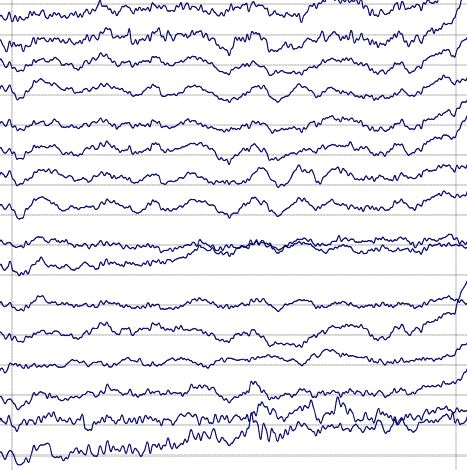
\includegraphics[width=6cm,height=6cm]{eeg.jpg}};

\pic[shift={(3,0,0)}] at (input-east) 
    {RightBandedBox={
        name=conv17,
        caption=conv1,
        xlabel=6,
        ylabel=28,
        zlabel=28,
        fill=\ConvColor,
        bandfill=\ConvReluColor,
        height=28,
        width=6,
        depth=28
        }
    };

\draw [connection]  (input-east)    -- node {\midarrow} (conv17-west);

\pic[shift={ (0,0,0) }] at (conv17-east) 
    {Box={
        name=pool1,
        caption=AvgPool,
        xlabel=6,
        ylabel=14,
        zlabel=14,    
        fill=\PoolColor,
        opacity=0.5,
        height=14,
        width=6,
        depth=14
        }
    };

\pic[shift={(2,0,0)}] at (pool1-east) 
    {RightBandedBox={
        name=conv2,
        caption=conv2,
        xlabel=8,
        ylabel=10,
        zlabel=10,
        fill=\ConvColor,
        bandfill=\ConvReluColor,
        height=10,
        width=8,
        depth=10
        }
    };

\draw [connection]  (pool1-east)    -- node {\midarrow} (conv2-west);

\pic[shift={ (0,0,0) }] at (conv2-east) 
    {Box={
        name=pool27,
        caption=AvgPool,
        xlabel=8,
        ylabel=5,
        zlabel=5,    
        fill=\PoolColor,
        opacity=0.5,
        height=5,
        width=8,
        depth=5
        }
    };

\pic[shift={(5,0,0)}] at (pool27-east) 
    {Box={
        name=input7,
        caption=frame1,
        xlabel=1,
        ylabel=1,
        zlabel=200,
        fill=\ConvColor,
        height=2.5,
        width=2.5,
        depth=100
        }
    };

\pic[shift={ (6,0,0) }] at (input7-east) 
    {Box={
        name=node17,
        caption=,
        xlabel=1,
        ylabel=1,
        zlabel=16,
        fill=\FcColor,
        height=2.5,
        width=2.5,
        depth=8
        }
    };

\pic[shift={ (3,0,0) }] at (node17-east) 
    {Box={
        name=node27,
        caption=,
        xlabel=1,
        ylabel=1,
        zlabel=16,
        fill=\FcColor,
        height=2.5,
        width=2.5,
        depth=8
        }
    };

\pic[shift={ (3,0,0) }] at (node27-east) 
    {Box={
        name=node37,
        caption=,
        xlabel=1,
        ylabel=1,
        zlabel=16,
        fill=\FcColor,
        height=2.5,
        width=2.5,
        depth=8
        }
    };

\draw [connection]  (pool27-east)    -- node {\midarrow} (input7-west);

\draw [connection]  (input7-east)    -- node {\midarrow} (node17-west);

\draw [connection]  (node17-east)    -- node {\midarrow} (node27-west);

\draw [connection]  (node27-east)    -- node {\midarrow} (node37-west);

\pic[shift={(0,4,0)}] at (node17-south) 
    {Ball={
        name=transNode12,
        fill=\SumColor,
        opacity=0,
        radius=0,
        logo=$+$
        }
    };

\pic[shift={(0,4,0)}] at (node27-south) 
    {Ball={
        name=transNode22,
        fill=\SumColor,
        opacity=0,
        radius=0,
        logo=$+$
        }
    };

\pic[shift={(0,4,0)}] at (node37-south) 
    {Ball={
        name=transNode32,
        fill=\SumColor,
        opacity=0,
        radius=0,
        logo=$+$
        }
    };

\draw [connection]  (transNode12-south)    -- node {\midarrow} (node17-north);

\draw [connection]  (transNode22-south)    -- node {\midarrow} (node27-north);

\draw [connection]  (transNode32-south)    -- node {\midarrow} (node37-north);

\pic[shift={(3,0,0)}] at (node37-east) 
    {Box={
        name=softMax,
        caption=SoftMax,
        xlabel=1,
        ylabel=1,
        zlabel=4,
        fill=\SoftmaxColor,
        opacity=0.5,
        height=2,
        width=2,
        depth=5
        }
    };

\draw [connection]  (node37-east)    -- node {\midarrow} (softMax-west);

\end{tikzpicture}
\end{document}
